\documentclass[conference]{IEEEtran}
\IEEEoverridecommandlockouts
\usepackage{cite}
\usepackage{amsmath,amssymb,amsfonts}
\usepackage{graphicx}
\usepackage{textcomp}
\usepackage{booktabs}
\usepackage{array}
\usepackage{float}
\usepackage{algorithm}
\usepackage{algpseudocode}
\usepackage{tikz}
\usepackage{pgfplots}
\pgfplotsset{compat=1.16}
\usepackage{url}
\def\UrlBreaks{\do\/\do\-\do\.\do\_}
\urlstyle{same}
\usetikzlibrary{shapes.geometric,shapes.misc,arrows.meta,positioning,fit,backgrounds,calc}
\usepackage[colorlinks=true,citecolor=blue,urlcolor=blue,linkcolor=black,bookmarks=false,pdftitle={SN-LPA: Size Normalized Label Propagation Algorithm},pdfauthor={Lakshay, Aman Tomar}]{hyperref}
\def\BibTeX{{\rm B\kern-.05em{\sc i\kern-.025em b}\kern-.08em T\kern-.1667em\lower.7ex\hbox{E}\kern-.125em X}}
\algrenewcommand\algorithmicrequire{\textbf{Input:}}
\algrenewcommand\algorithmicensure{\textbf{Output:}}
\algrenewcommand\alglinenumber[1]{\scriptsize #1:}
\newcommand{\algcomment}[1]{\Statex \textit{// #1}}
\DeclareMathOperator*{\argmax}{arg\,max}
\newcommand{\metrichead}[1]{\par\smallskip\noindent\textbf{#1}\par\nobreak\vspace{1pt}}

% ---------- flowchart styles (ISO 5807 symbols: oval = start/end, rectangle = process, diamond = decision, parallelogram = input/output)
\tikzset{
  term/.style={rounded rectangle, draw, thick, font=\scriptsize, minimum height=5mm, minimum width=12mm, fill=gray!12},
  io/.style={trapezium, trapezium left angle=72, trapezium right angle=108, draw, thick, font=\scriptsize, align=center, minimum height=6.5mm, fill=gray!8},
  proc/.style={rectangle, draw, thick, font=\scriptsize, align=center, minimum height=7mm, inner sep=2.5pt},
  dec/.style={diamond, aspect=2.4, draw, thick, font=\scriptsize, align=center, inner sep=1.5pt},
  newp/.style={proc, fill=blue!14},
  modp/.style={proc, fill=orange!28},
  arr/.style={-{Stealth[length=1.8mm,width=1.5mm]}, thick},
  lab/.style={font=\scriptsize\itshape, inner sep=1pt}
}

\begin{document}

\title{SN-LPA: Size Normalized Label Propagation Algorithm}

\author{%
\begin{tabular}[t]{c}
Lakshay (2023UCA1838)\\[0.5ex]
{\small\textit{Dept.\ of Computer Science and Engineering}}\\
{\small\textit{Netaji Subhas University of Technology (NSUT)}}\\
{\small New Delhi, India}
\end{tabular}%
\hspace{2.2cm}%
\begin{tabular}[t]{c}
Aman Tomar (2023UCA1818)\\[0.5ex]
{\small\textit{Dept.\ of Computer Science and Engineering}}\\
{\small\textit{Netaji Subhas University of Technology (NSUT)}}\\
{\small New Delhi, India}
\end{tabular}\\[3ex]
\begin{tabular}[t]{c}
Under the supervision of Dr.\ Vandana Bhatia\\[0.5ex]
{\small\textit{Dept.\ of Computer Science and Engineering}}\\
{\small\textit{Netaji Subhas University of Technology (NSUT)}}\\
{\small New Delhi, India}
\end{tabular}
}

\maketitle

\begin{abstract}
Label propagation finds communities in near-linear time, but it is unstable and blind to resolution. TPOC-LPA (Kong et al., 2026) is a recent three-stage variant that seeds communities from node importance, evolves labels by an attractiveness score, and filters labels to allow overlap. We re-implement it and find that its Stage~2 score sums neighbour attractiveness with no size normalisation, so a growing community is rewarded for size alone: on a dense graph (email-Eu) it collapses to one community (NMI 0.00), and on sparse graphs it under-merges. We propose SN-LPA (Size Normalized Label Propagation Algorithm): six modifications, all optional and off by default so that the default behaviour is the published algorithm: a triangle-based similarity, a best-iterate guard, a size-corrected gain, a label-free granularity rule that chooses between the two regimes, a merge pass that stops at the minimum of the map equation, and boundary-node moves scored by the Synwalk objective. We compare SN-LPA with Fastgreedy, LPA, Louvain and Walktrap, re-run on identical graphs, plus Infomap as an extra. It has the best mean rank on 11 real networks and the highest mean NMI on six LFR settings (0.9941 against 0.9905 for Infomap), but it is far behind Infomap on SNAP-Youtube. On overlapping LFR graphs it beats SLPA on four of six families and loses on the two largest, and on the extended modularity EQ it wins on 5 of 12 real networks against SLPA. We also report the ideas that failed and the limits we could not remove.
\end{abstract}

\begin{IEEEkeywords}
community detection, label propagation, overlapping communities, map equation, resolution limit, node importance
\end{IEEEkeywords}

%=====================================================================
\section{Introduction}\label{sec:intro}
\subsection{Background and Motivation}
Many real systems are networks: people and their friendships, authors and their co-authorships, proteins and their interactions, web pages and their links. A recurring feature of such networks is \emph{community structure}: the nodes fall into groups that are densely connected inside and sparsely connected to the rest~\cite{girvan2002,fortunato2010}. Finding these groups, called community detection, helps to understand how a network is organised, to predict missing links and attributes, and to summarise a graph that is too large to inspect. The task is hard to define exactly, so a large number of methods exist: they optimise modularity~\cite{newman2004}, simulate random walks~\cite{pons2006,rosvall2008}, or let nodes exchange labels~\cite{raghavan2007}.

Label propagation algorithms (LPA) are among the cheapest of these. Every node starts with its own label and repeatedly adopts the label that is most common among its neighbours; connected groups converge to a shared label. One pass costs $O(m)$ for a graph with $m$ edges, there is no parameter to set, and the number of communities need not be known. This is why LPA and its descendants are used on graphs with millions of edges~\cite{leung2009,traag2023}. The price is quality. Plain LPA is non-deterministic because ties are broken at random, it can converge to very different partitions on different runs, and on some graphs a single label takes over the whole network~\cite{raghavan2007}.

\subsection{From Label Propagation to TPOC-LPA}
A long line of work therefore adds structure to the propagation rule. Some methods replace the majority vote by a modularity gain~\cite{barber2009} and merge communities afterwards~\cite{liu2010}. Others fix the order in which nodes are updated, or weight the votes by how important a node is in the graph. A second need is \emph{overlap}: a person belongs to several social circles, a protein to several complexes, and a method that assigns each node to exactly one group cannot express this. Overlapping variants let a node keep several labels~\cite{gregory2010,xie2011}.

TPOC-LPA~\cite{kong2026} is a recent method that combines these ideas in three stages. Stage~1 seeds communities around nodes of high \emph{importance}, growing each by a tightness--sparsity test. Stage~2 lets every node adopt the community that attracts it most, where the attraction combines neighbour importance with a neighbourhood-similarity term. Stage~3 filters the labels of nodes that touch several communities, so that a node keeps more than one label only if its affiliation to each is strong enough. The paper reports the best average NMI among seven methods on eight real networks, the best NMI on all six of its LFR benchmarks, and the best extended modularity on most of 12 real networks for overlap. We took it as our starting point.

\subsection{What We Observed}
We re-implemented the algorithm from the paper, checked every formula against the worked examples in it, and then tested it beyond the graphs it reports. Two behaviours stand out. First, on a dense graph (email-Eu-core: 986 nodes, 42 departments, average degree 33) Stage~1 gives 335 communities at NMI 0.54, and Stage~2 then merges all of them into a single community, so NMI drops to 0.00. On LFR graphs with a realised mixing parameter of $\mu=0.7$ the NMI averages 0.05. Second, on sparse graphs the opposite happens: on Cora Stage~2 leaves 214 communities for 7 classes. The cause is in the Stage~2 score (Eq.~\eqref{eq:stage2} below): it sums neighbour attractiveness with no term that depends on community size, so a community that grows is rewarded for its size alone.

\subsection{Research Gap}\label{sec:gap}
From this reading and from our experiments we identify the following gaps.
\begin{enumerate}
\item \textbf{No analysis of the size effect in Stage~2.} Label propagation with an unnormalised score is known to be unstable; modularity-specialised variants fix it with a null-model term~\cite{barber2009}. TPOC-LPA does not include such a term, and its behaviour on dense graphs and on graphs with high mixing was not studied; the benchmark graphs in the paper are those where the rule works.
\item \textbf{Resolution is not controlled.} The propagation stops at a local fixed point with no check of the scale of the communities. Merge steps that exist in related work use modularity, whose resolution limit depends on the size of the whole network~\cite{fortunato2007}, and we show that this can destroy a good partition (Sec.~\ref{sec:results}).
\item \textbf{Missing strong baselines and reproducibility.} The comparison in~\cite{kong2026} omits methods based on the map equation, and six of its baselines (NSA, SimCMR, WLC, UMSTMO, GREESE, MDPA) have no public implementation that we could find. Published numbers for them cannot be checked, and the choice of the NMI normalisation is not stated.
\item \textbf{The overlap rate is not calibrated.} The affiliation threshold $\beta$ is a fixed parameter, and nothing relates it to how many nodes of a given graph should be overlapping.
\item \textbf{Where a change helps and where it hurts is rarely reported.} Improvements to label propagation are usually shown on the graphs they were designed for. A change that helps on one family of graphs can hurt on another, and this needs a protocol with development and held-out graphs.
\end{enumerate}

\subsection{Contributions}\label{sec:contrib}
\begin{enumerate}
\item \textbf{Diagnosis.} We re-implement TPOC-LPA and show that its Stage~2 rule is the $\gamma{=}0$ end of a size-corrected family, which explains both the collapse on dense graphs and the under-merging on sparse ones (Sec.~\ref{sec:problem}).
\item \textbf{SN-LPA, a pipeline of six optional modifications (M1--M6),} with the published behaviour as the default: triangle similarity, best-iterate guard, size-corrected gain, a label-free granularity rule that chooses between the two regimes, a merge pass stopped by the map equation, and boundary moves scored by the Synwalk objective with a regularised acceptance gate. The ideas come from existing work; the specific combination, the rule and the gate are ours (Sec.~\ref{sec:arch}). We give the algorithm in pseudocode (Algorithms~\ref{alg:base}--\ref{alg:moves}).
\item \textbf{A like-for-like comparison.} We re-run the baselines of~\cite{kong2026} that have public code, plus Infomap, on identical graphs with identical metric code, and report wins and losses, including the results that do not favour us (Sec.~\ref{sec:results}).
\item \textbf{Negative results and limits.} We report the ideas that failed and the gaps we could not close (Sec.~\ref{sec:discussion}).
\end{enumerate}

\subsection{Organisation}
Section~II reviews related work. Section~III describes the datasets, the evaluation metrics, the baseline, its problems and the proposed architecture. Section~IV presents the results, Section~V discusses them, and Section~VI concludes.

%=====================================================================
\section{Related Work and Literature Review}\label{sec:related}
\subsection{Community Detection: Objectives and Families}
Girvan and Newman~\cite{girvan2002} popularised community detection with a divisive method and with the football and karate networks as test cases; Fortunato~\cite{fortunato2010} surveys the field. Methods differ by what they optimise. \emph{Modularity}-based methods maximise the difference between the number of edges inside communities and its expectation in a degree-preserving random graph~\cite{newman2004}: Fastgreedy~\cite{clauset2004} merges communities greedily, and Louvain~\cite{blondel2008} alternates local moves with aggregation. Leiden~\cite{traag2019} refines Louvain to guarantee connected communities (we did not run it). \emph{Random-walk} methods use the idea that a walker stays inside a community for a long time: Walktrap~\cite{pons2006} clusters nodes by walk distances, and the map equation~\cite{rosvall2008} minimises the code length of a walker's path. Lancichinetti and Fortunato~\cite{lancichinetti2009cmp} compare many of these methods on benchmark graphs.

\subsection{Label Propagation and its Variants}
Raghavan et al.~\cite{raghavan2007} introduced the majority-vote rule. Leung et al.~\cite{leung2009} analysed its behaviour on large networks and proposed ways to stabilise it. Traag and \v{S}ubelj~\cite{traag2023} make label propagation faster by processing only nodes whose neighbourhood changed. LPAm~\cite{barber2009} derives a label update from modularity: the gain of joining community $c$ is the number of links into $c$ minus the number expected under the configuration model. LPAm can get stuck in poor local optima, and LPAm+~\cite{liu2010} adds a multistep greedy merge of communities to escape them, in the spirit of~\cite{clauset2004}. Li et al.~\cite{li2020motif} weight propagation by motifs (triangles), which motivates our similarity.

\subsection{Overlapping Community Detection}
The clique percolation method of Palla et al.~\cite{palla2005} made overlap a central topic. In label propagation, COPRA~\cite{gregory2010} lets each node hold several labels with belonging coefficients, and SLPA~\cite{xie2011} stores the labels a node has received over $T$ rounds and keeps those whose relative frequency exceeds a threshold $r$; it is the best known overlapping label-propagation baseline and we use it. Ego-splitting~\cite{epasto2017} clusters a graph whose nodes are the ``personas'' of each node. TPOC-LPA~\cite{kong2026} filters labels by a weighted affiliation score (WAS) and keeps those above a threshold times the node's mean score.

\subsection{Resolution Limit, Map Equation and Random-Walk Objectives}
Fortunato and Barth\'elemy~\cite{fortunato2007} showed that modularity cannot resolve communities smaller than a scale that depends on the total number of links in the network. The map equation~\cite{rosvall2008} avoids this: Kawamoto and Rosvall~\cite{kawamoto2015} derive that its resolution limit is set by the number of links \emph{between} modules instead. On sparse networks the map equation tends to over-fit, which regularised versions address with a prior on unobserved links~\cite{smiljanic2020}. Synwalk~\cite{toth2022} fits a random-walk model to a partition and is reported to outperform Infomap on networks with high mixing. These three results are what our merge stop (M5) and boundary moves (M6) rest on.

\subsection{TPOC-LPA and Where We Stand}
Table~\ref{tab:related} summarises how the methods above relate to this work. TPOC-LPA~\cite{kong2026} combines node importance, a CTS-gated pre-selection and WAS filtering, but it has no size correction, no resolution control and no calibrated overlap rate. We keep all of its stages and replace or extend the middle of the pipeline.
\begin{table}[H]
\centering
\caption{Related methods and their role in this work.}
\label{tab:related}
\scriptsize
\begin{tabular}{>{\raggedright\arraybackslash}p{19mm}>{\raggedright\arraybackslash}p{26mm}>{\raggedright\arraybackslash}p{29mm}}
\toprule
Method & Key idea & Used here as \\
\midrule
LPA~\cite{raghavan2007} & Majority label vote & Baseline (run) \\
LPAm / LPAm+~\cite{barber2009,liu2010} & Modularity gain; greedy merge & Size-corrected gain (M3); merge order (M5) \\
Li et al.~\cite{li2020motif} & Triangle-weighted propagation & Motivation for M1 \\
Louvain, Fastgreedy~\cite{blondel2008,clauset2004} & Modularity optimisation & Baselines (run) \\
Walktrap~\cite{pons2006} & Walk distances & Baseline (run) \\
Infomap~\cite{rosvall2008,kawamoto2015,smiljanic2020} & Map equation; resolution limit; regularisation & Extra baseline; merge stop (M5); gate (M6) \\
Synwalk~\cite{toth2022} & Walk-model objective $J$ & Move score (M6) \\
SLPA~\cite{xie2011} & Label memory, threshold $r$ & Overlap baseline (run) \\
TPOC-LPA~\cite{kong2026} & NI seeds, CTS, WAS & Baseline (re-implemented) \\
\bottomrule
\end{tabular}
\end{table}
\textbf{Sourcing note.} The cited methods support the ideas we use; they do not show that the ideas work inside TPOC-LPA. That evidence is our experiments, including the ones that failed. We read several of the cited papers only in part (the abstracts and the sections defining the objectives we use), and we had no access to the full text of~\cite{li2020motif}.

%=====================================================================
\section{Methodology}\label{sec:method}
\subsection{Datasets}\label{sec:data}
We use four groups of graphs. All graphs are treated as undirected and unweighted. (We found that the Karate graph shipped with networkx carries edge weights; we removed them, see Sec.~\ref{sec:discussion}.)

\textbf{Real networks with ground truth.} Table~\ref{tab:data} lists them: Karate~\cite{zachary1977}, Dolphin (four groups reconstructed from the original study~\cite{lusseau2003}), Football~\cite{girvan2002} (conferences), Polbooks (political leaning), Polblogs~\cite{adamic2005}, email-Eu-core (departments, from~\cite{yin2017}), Cora and Citeseer~\cite{sen2008} (paper classes), and three SNAP graphs with ground-truth communities~\cite{yang2012}. The SNAP graphs are our own induced subgraphs, $2.6$--$3.9\times$ larger than the subsets used in~\cite{kong2026}, with the first listed community as the label of each node; absolute values are therefore not comparable to the paper, only across our columns. Karate to Citeseer use the largest connected component.
@@T_DATA@@

\textbf{LFR benchmarks (disjoint).} We use the generator of Lancichinetti et al.~\cite{lfr2008} with the six settings of~\cite{kong2026} (Table~\ref{tab:lfrparam}): average degree 20, power-law exponents $\tau_1=3$, $\tau_2=1.5$, mixing $\mu\in\{0.1,0.6\}$. The generator in networkx realises a mixing far above its nominal value (nominal 0.6 gives about 0.84), so we search the nominal value until the \emph{realised} mixing equals the target. For $n=1000$ the minimum community size is 15 instead of 10, since 10 is infeasible with degree 20 in this generator. Five graphs (seeds 1--5) are generated per setting.
\begin{table}[H]
\centering
\caption{LFR settings for disjoint communities.}
\label{tab:lfrparam}
\scriptsize
\begin{tabular}{lrrrr}
\toprule
Name & $n$ & $k_{\max}$ & $c_{\min}$--$c_{\max}$ & $\mu$ \\
\midrule
N1 / N2 & 1000 & 50 & 15--50 & 0.1 / 0.6 \\
N3 / N4 & 5000 & 50 & 20--100 & 0.1 / 0.6 \\
N5 / N6 & 10000 & 100 & 20--200 & 0.1 / 0.6 \\
\bottomrule
\end{tabular}
\end{table}

\textbf{LFR benchmarks (overlapping).} The six families R1--R6 of Table~7 in~\cite{kong2026}: $n\in\{1000,5000,10000\}$, $\mu\in\{0.1,0.3\}$, average degree 10 (20 for $n=10000$), and $om\in\{2,\dots,8\}$ memberships for the overlapping nodes ($on=100,500,2000$ of them); 42 graphs per seed, two seeds, from the original generator of Lancichinetti et al.

\textbf{Networks for EQ.} Karate, Dolphin, Lesmis, Jazz, Cora (2708 nodes), Power, Facebook, CA-GrQc, LastFM-Asia, CA-HepTh, PGP and Deezer. Eleven of the twelve match the node and edge counts in~\cite{kong2026} (CA-GrQc and CA-HepTh differ by two nodes).

\subsection{Evaluation Metrics}\label{sec:metrics}
We report two kinds of metrics. \emph{External} metrics compare a detected result $X$ with the ground truth $Y$ and measure agreement; \emph{internal} metrics (modularity, EQ) need no ground truth and measure how well the result fits the graph's own structure. The two can disagree: a partition with higher modularity can match the truth worse, as we show on Karate. Throughout, $N$ is the number of nodes and $m$ the number of edges; all scores are better when higher. Table~\ref{tab:metrics} gives an overview, and the rest of this subsection explains each metric and gives its definition.
\begin{table}[H]
\centering
\caption{Evaluation metrics.}
\label{tab:metrics}
\scriptsize
\setlength{\tabcolsep}{3pt}
\begin{tabular}{llcc}
\toprule
Metric & Result type & Needs truth & Range \\
\midrule
NMI & disjoint & yes & $[0,1]$ \\
Modularity $Q$ & disjoint & no & $\le 1$ \\
LFK-NMI & overlapping & yes & $[0,1]$ \\
$\mathrm{NMI}_{\max}$ & overlapping & yes & $[0,1]$ \\
Omega index & overlapping & yes & $\le 1$ \\
EQ & overlapping & no & $\le 1$ \\
\bottomrule
\end{tabular}
\end{table}

\metrichead{1) Normalised Mutual Information (NMI)}
NMI asks how much knowing a node's detected community tells us about its true community. It is the mutual information of the two labelings, divided by their entropies so that the score lies in $[0,1]$: 1 for identical partitions and close to 0 for unrelated ones. It ignores how communities are named, and the two partitions need not have the same number of communities. With $n_k$ the size of community $k$,
\begin{equation}
\mathrm{NMI}(X,Y)=\frac{2\,I(X;Y)}{H(X)+H(Y)},\label{eq:nmi}
\end{equation}
where $H(X)=-\sum_k\frac{n_k}{N}\log\frac{n_k}{N}$ and $I(X;Y)=H(X)+H(Y)-H(X,Y)$. We use this arithmetic normalisation in every column of our tables (see Sec.~\ref{sec:setup}).

\metrichead{2) Modularity ($Q$)}
Modularity compares the fraction of edges inside communities with the fraction expected if the same nodes were wired at random while keeping their degrees. A high value means many more internal edges than chance would give. It needs no ground truth, but it has a resolution limit~\cite{fortunato2007}, so a high $Q$ does not guarantee that communities match the truth.
\begin{equation}
Q=\frac1{2m}\sum_{u,w}\Big(A_{uw}-\frac{k_uk_w}{2m}\Big)\,\delta(c_u,c_w),\label{eq:Q}
\end{equation}
where $A$ is the adjacency matrix, $k_u$ the degree of $u$, and $\delta(c_u,c_w)=1$ if $u$ and $w$ share a community. We compute $Q$ on the unweighted graph.

\metrichead{3) LFK-NMI and $\mathrm{NMI}_{\max}$ (overlapping covers)}
NMI assumes that every node has one label. For covers, Lancichinetti et al.~\cite{lfk2009} treat each community $X_k$ as a yes/no variable (``is this node in $X_k$?'') with entropy
\begin{equation}
H(X_k)=h(p_k)+h(1-p_k),\qquad p_k=\frac{|X_k|}{N},
\end{equation}
where $h(p)=-p\log_2p$.
How much the other cover $Y$ tells us about $X_k$ is measured through its best-matching community,
\begin{equation}
H(X_k|Y)=\min_lH(X_k|Y_l),
\end{equation}
taken over those $Y_l$ that satisfy the constraint of~\cite{lfk2009} (a match counts only if it is better than chance). LFK-NMI averages this over the communities, each normalised by its own entropy:
\begin{align}
\tilde H(X|Y)&=\frac1{|X|}\sum_k\frac{H(X_k|Y)}{H(X_k)},\label{eq:lfk1}\\
\mathrm{NMI}_{\mathrm{LFK}}&=1-\tfrac12\big[\tilde H(X|Y)+\tilde H(Y|X)\big].\label{eq:lfk}
\end{align}
The variant $\mathrm{NMI}_{\max}$ sums the entropies instead and divides by the larger one, which is stricter:
\begin{align}
I(X\!:\!Y)&=\tfrac12\big[H(X)+H(Y)-H(X|Y)-H(Y|X)\big],\\
\mathrm{NMI}_{\max}&=\frac{I(X\!:\!Y)}{\max\{H(X),H(Y)\}},
\end{align}
with $H(X)=\sum_kH(X_k)$ and $H(X|Y)=\sum_kH(X_k|Y)$.

\metrichead{4) Omega index}
Omega is a pair-counting measure. For every pair of nodes it counts in how many communities the pair appears together, and checks whether the detected and the true cover give the same count. It generalises the Rand index to overlapping covers~\cite{collins1988}; the correction for chance makes 0 mean ``no better than random''. Let $t_X(p)$ be the number of communities of $X$ that contain both nodes of pair $p$, and $N_p=\binom N2$. Then
\begin{equation}
\Omega=\frac{\Omega_u-\Omega_e}{1-\Omega_e},\qquad\Omega_u=\frac1{N_p}\sum_p\mathbf 1\big[t_X(p)=t_Y(p)\big],\label{eq:omega}
\end{equation}
and $\Omega_e=\sum_jA_jB_j/N_p^2$ is the agreement expected by chance, where $A_j$ ($B_j$) is the number of pairs with $t_X=j$ ($t_Y=j$). For partitions $\Omega$ equals the adjusted Rand index; we checked this numerically.

\metrichead{5) Extended modularity (EQ)}
EQ extends modularity to covers~\cite{shen2009}. A node in $O_u$ communities contributes to each of them with weight $1/O_u$, so overlap is not counted twice. It needs no ground truth, it equals $Q$ for partitions, and it is the measure used in~\cite{kong2026} for overlapping results on real networks.
\begin{equation}
\mathrm{EQ}=\frac1{2m}\sum_c\sum_{u,w\in c}\frac{1}{O_uO_w}\Big(A_{uw}-\frac{k_uk_w}{2m}\Big).\label{eq:eq}
\end{equation}
Evaluated directly this costs $O(\sum_c|c|^2)$. We use the equivalent form
\begin{equation}
\begin{split}
\mathrm{EQ}&=\frac1{2m}\sum_{(u,w)\in E}\frac{2\,s_{uw}}{O_uO_w}\\
&\quad-\frac1{2m}\sum_c\frac{S_c^{2}}{2m},
\end{split}
\end{equation}
with $s_{uw}$ the number of communities shared by $u$ and $w$, and $S_c=\sum_{u\in c}k_u/O_u$. It costs $O(m)$, and we verified it against the direct sum.

\subsection{Baseline: TPOC-LPA}\label{sec:base}
Fig.~\ref{fig:base} shows the architecture and Algorithm~\ref{alg:base} the pseudocode, which follows Algorithm~1 of~\cite{kong2026}. 

\textbf{Node importance.} For node $i$ with degree $d_i$ and $c_i$ edges among its neighbours, $f_i=d_i\,(1+c_i/\sum_kc_k)$ is min--max scaled to $e_i=0.5+0.5\,\frac{f_i-f_{\min}}{f_{\max}-f_{\min}}$, and
\begin{equation}
NI(i)=e_i+\frac1{|N(i)|}\sum_{j\in N(i)}e_j.\label{eq:ni}
\end{equation}

\textbf{Stage 1: pre-selection.} The unlabelled node with the largest $NI$ becomes a core. Its unlabelled neighbours are visited in decreasing $NI$; a neighbour joins if the tightness--sparsity value of the community, $\mathrm{CTS}=c_t/(1+c_s)$ with $c_t=e_{in}/n_c$ and $c_s=e_{out}/(e_{in}+e_{out})$, does not fall below $\alpha$ times its previous value. This repeats until every node has a label.

\textbf{Stage 2: evolution.} The attractiveness of an edge is
\begin{equation}
A(i,j)=\frac{NI(i)\,NI(j)}{(2-\mathrm{Sim}(i,j))^2},\quad \mathrm{Sim}(i,j)=\frac{|N(i)\cap N(j)|}{|N(i)\cup N(j)|}.\label{eq:A}
\end{equation}
In decreasing $NI$ order, node $i$ takes the community
\begin{equation}
c^{*}(i)=\argmax_{c}\;\sum_{j\in N(i)\cap c}A(i,j),\label{eq:stage2}
\end{equation}
(directly the only one if all neighbours share a label) until no label changes or $max\_iter$ is reached.

\textbf{Stage 3: label filtering.} The weighted affiliation of node $i$ to a label $c$ present among its neighbours is
\begin{equation}
\mathrm{WAS}(i,c)=\frac{\sum_{j\in N(i),\,\ell(j)=c}NI(j)}{\sum_{k\in N(i)}NI(k)},\label{eq:was}
\end{equation}
and $i$ keeps, besides its own label, every $c$ with $\mathrm{WAS}(i,c)\ge\beta\cdot\overline{\mathrm{WAS}}(i)$ ($\beta=0.8$), where the bar is the mean over the labels present.

\begin{algorithm}[t]
\footnotesize
\caption{TPOC-LPA (baseline, after~\cite{kong2026})}\label{alg:base}
\begin{algorithmic}[1]
\Require $G=(V,E)$, $\alpha$, $\beta$, $max\_iter$
\Ensure Overlapping community set $Communities$
\algcomment{Step 1: community pre-selection}
\For{all $i\in V$} compute $NI(i)$ by Eq.~\eqref{eq:ni} \EndFor
\State $U\gets V$
\While{$U\neq\emptyset$}
  \State $u\gets\argmax_{x\in U}NI(x)$; $label(u)\gets u$; $U\gets U\setminus\{u\}$
  \State $s\gets\{u\}$; $CTS_{prev}\gets0$
  \For{all neighbours $v\in U$ of $u$ in descending $NI(v)$}
    \State compute $CTS_{curr}$ of $s\cup\{v\}$
    \If{$CTS_{curr}\ge\alpha\cdot CTS_{prev}$}
      \State $s\gets s\cup\{v\}$; $label(v)\gets u$
      \State $U\gets U\setminus\{v\}$; $CTS_{prev}\gets CTS_{curr}$
    \EndIf
  \EndFor
\EndWhile
\algcomment{Step 2: community evolution}
\State $iter\gets0$
\Repeat
  \For{all $i\in V$ in descending $NI(i)$}
    \State $RC\gets\{label(j):j\in N(i)\}$
    \If{$|RC|=1$} \State $label(i)\gets$ the label in $RC$
    \Else \State $label(i)\gets\argmax_{c\in RC}\sum_{j\in N(i)\cap c}A(i,j)$
    \EndIf
  \EndFor
  \State $iter\gets iter+1$
\Until{no label changed \textbf{or} $iter=max\_iter$}
\algcomment{Step 3: community label filtering}
\For{all $i\in V$} $Communities[i]\gets\{label(i)\}$ \EndFor
\For{all $i\in V$}
  \State $CL\gets\{label(j):j\in N(i)\}$
  \If{$|CL|>1$}
    \State compute $\mathrm{WAS}(i,c)$, $c\in CL$ (Eq.~\eqref{eq:was})
    \State $\overline{\mathrm{WAS}}\gets$ mean of these values
    \State $V_i\gets\{c\in CL:\mathrm{WAS}(i,c)\ge\beta\,\overline{\mathrm{WAS}}\}$
    \State $Communities[i]\gets Communities[i]\cup V_i$
  \EndIf
\EndFor
\State \Return $Communities$
\end{algorithmic}
\end{algorithm}

\begin{figure}[t]
\centering
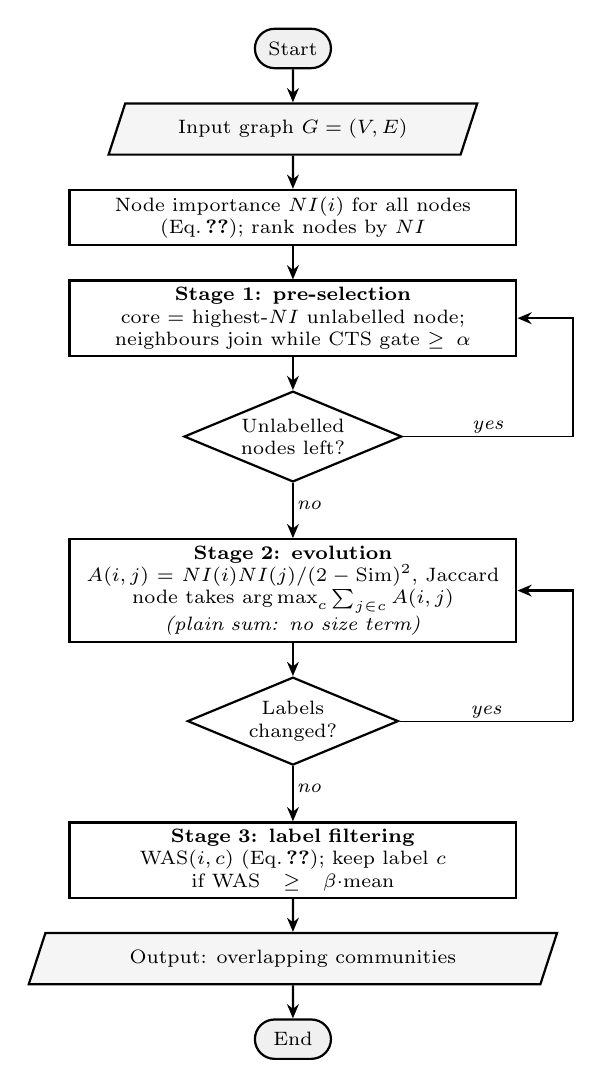
\begin{tikzpicture}[node distance=4.2mm]
\node[term] (s) {Start};
\node[io, below=of s] (in) {Input graph $G=(V,E)$};
\node[proc, below=of in, text width=55mm] (ni) {Node importance $NI(i)$ for all nodes\\(Eq.\,\ref{eq:ni}); rank nodes by $NI$};
\node[proc, below=of ni, text width=55mm] (s1) {\textbf{Stage 1: pre-selection}\\ core = highest-$NI$ unlabelled node;\\ neighbours join while CTS gate $\ge\alpha$};
\node[dec, below=of s1] (d1) {Unlabelled\\nodes left?};
\node[proc, below=7mm of d1, text width=55mm] (s2) {\textbf{Stage 2: evolution}\\ $A(i,j)=NI(i)NI(j)/(2-\mathrm{Sim})^2$, Jaccard\\ node takes $\argmax_c\sum_{j\in c}A(i,j)$\\ \textit{(plain sum: no size term)}};
\node[dec, below=of s2] (d2) {Labels\\changed?};
\node[proc, below=7mm of d2, text width=55mm] (s3) {\textbf{Stage 3: label filtering}\\ $\mathrm{WAS}(i,c)$ (Eq.\,\ref{eq:was}); keep label $c$\\ if $\mathrm{WAS}\ge\beta\cdot$mean};
\node[io, below=of s3] (out) {Output: overlapping communities};
\node[term, below=of out] (e) {End};
\draw[arr] (s)--(in); \draw[arr] (in)--(ni); \draw[arr] (ni)--(s1); \draw[arr] (s1)--(d1);
\draw[arr] (d1)--(s2) node[lab, pos=.4, right]{no};
\coordinate (p1) at ($(d1.east -| s1.east)+(7mm,0)$);
\draw (d1.east) -- (p1) node[lab, pos=.5, above]{yes};
\draw[arr] (p1) -- (p1 |- s1.east) -- (s1.east);
\draw[arr] (s2)--(d2);
\draw[arr] (d2)--(s3) node[lab, pos=.4, right]{no};
\coordinate (p2) at ($(d2.east -| s2.east)+(7mm,0)$);
\draw (d2.east) -- (p2) node[lab, pos=.5, above]{yes};
\draw[arr] (p2) -- (p2 |- s2.east) -- (s2.east);
\draw[arr] (s3)--(out); \draw[arr] (out)--(e);
\end{tikzpicture}
\caption{Architecture of the baseline TPOC-LPA~\cite{kong2026}. Oval = start/end, parallelogram = input/output, rectangle = process, diamond = decision.}
\label{fig:base}
\end{figure}

\subsection{Problems with the Baseline}\label{sec:problem}
Reading Algorithm~\ref{alg:base} against our experiments, we find the following problems.
\begin{enumerate}
\item \textbf{Unbounded size effect (collapse).} Eq.~\eqref{eq:stage2} adds up neighbour attractiveness. If community $c$ has $n_c$ nodes, a node adjacent to it tends to have more neighbours inside $c$ as $n_c$ grows, so $\sum_{j\in c}A(i,j)$ tends to grow with the size of $c$ alone. The larger community then attracts more nodes, which makes it larger: a rich-get-richer dynamic with nothing that bounds it. On email-Eu this runs away: Stage~1 gives 335 communities at NMI 0.5415 and Stage~2 ends with one community and NMI 0.0000. On LFR graphs with realised $\mu=0.7$ the average NMI is 0.05.
\item \textbf{Under-merging on sparse graphs.} When degrees are low, a node has few neighbours in any community and the sum is small, so fragments from Stage~1 do not merge. On Cora the baseline ends with 214 communities for 7 classes.
\item \textbf{The rule is only one end of a family.} Eq.~\eqref{eq:stage2} is the $\gamma=0$ end of
\begin{equation}
\mathrm{gain}(c)=\sum_{j\in N(i)\cap c}A(i,j)-\gamma\,\frac{s_i\,S_c}{W},\label{eq:gain}
\end{equation}
where $s_i=\sum_jA(i,j)$, $S_c=\sum_{k\in c}s_k$ and $W=\sum_is_i$. The subtracted term is the attraction expected in a random graph with the same strengths; it grows with $S_c$ and so bounds the effect in item~1. $\gamma=1$ is the LPAm gain~\cite{barber2009} with importance-weighted edges. No single $\gamma$ suits all graphs: a sweep of $\gamma$ from 0.1 to 0.75 found none that works in both regimes.
\item \textbf{The similarity can under-score tight communities.} Two well-connected nodes of one community share many neighbours but have a large union, so Jaccard in Eq.~\eqref{eq:A} gives a low value for a strong link.
\item \textbf{The last iterate is not always the best.} Stage~2 stops at a fixed point, which can be its worst round (the collapse in item~1).
\item \textbf{No control of the scale after Stage~2.} Nothing merges fragments at the right scale, and the only merge steps in related work use modularity, whose resolution limit can destroy a good partition (Sec.~\ref{sec:results}).
\item \textbf{Boundary nodes are not repaired.} Label propagation is least reliable at community boundaries, and nothing re-examines those nodes afterwards. On LFR graphs most of the remaining error is boundary nodes; at $\mu=0.6$ about half of the misplaced nodes have more links into another true community than into their own, so some of this error cannot be removed by any local rule.
\item \textbf{The overlap rate is fixed by $\beta$.} Stage~3 uses the same threshold on every graph (we return to this in Sec.~\ref{sec:discussion}).
\end{enumerate}

\subsection{Proposed Methodology}\label{sec:arch}
Fig.~\ref{fig:ours} shows the architecture of the proposed pipeline, SN-LPA (Size Normalized Label Propagation Algorithm); its central change is the size-normalised Stage~2 gain (M3). Stage~1 and Stage~3 of Algorithm~\ref{alg:base} are unchanged; Stage~2 is modified and two new steps follow it. The six modifications M1--M6 address problems 4, 5, 1--2, 3, 6 and 7 of Sec.~\ref{sec:problem}, respectively. Every option defaults to off, so the default code path is Algorithm~\ref{alg:base}. In the code they are labelled CHANGE 1, 2, 3, 4, 6 and 9. The pseudocode is given in Algorithms~\ref{alg:ours}--\ref{alg:moves}, in the same style as Algorithm~\ref{alg:base}.

\noindent Here \textsc{Evolve}$(L_1,\gamma)$ denotes Stage~2 started from the Stage~1 partition $L_1$, with the gain of Eq.~\eqref{eq:gain}; $\gamma=0$ gives Eq.~\eqref{eq:stage2}.

\begin{algorithm}[!t]
\footnotesize
\caption{Proposed pipeline (M1--M6)}\label{alg:ours}
\begin{algorithmic}[1]
\Require $G=(V,E)$, $\alpha$, $\beta$, $\gamma{=}1$, $\rho{=}1.5$, $max\_iter$, sweeps $S{=}20$
\Ensure Disjoint partition $L$, overlapping set $Communities$
\algcomment{Step 1: pre-selection (unchanged)}
\State $L_1\gets$ result of Step 1 of Algorithm~\ref{alg:base}
\algcomment{Step 2$'$: community evolution (modified)}
\State $\mathrm{Sim}(i,j)\gets c_{ij}/(1+c_{ij})$ for all edges \Comment{M1}
\State $L^{(0)}\gets\textsc{Evolve}(L_1,\gamma{=}0)$ \Comment{Eq.~\eqref{eq:stage2}}
\State \hspace{\algorithmicindent}keep the round with the largest $Q$ \Comment{M2}
\State $L^{(1)}\gets\textsc{Evolve}(L_1,\gamma{=}1)$ \Comment{M3, Eq.~\eqref{eq:gain}}
\If{$|L^{(1)}|\le\rho\,|L^{(0)}|$} \Comment{M4, Eq.~\eqref{eq:gran}}
  \State $L\gets L^{(1)}$
\Else
  \State $L\gets L^{(0)}$
\EndIf
\State $L\gets\textsc{MapEqMerge}(G,L)$ \Comment{M5, Alg.~\ref{alg:merge}}
\State $L\gets\textsc{SynwalkMoves}(G,NI,L,S)$ \Comment{M6, Alg.~\ref{alg:moves}}
\algcomment{Step 3: community label filtering (unchanged)}
\For{all $i\in V$} $Communities[i]\gets\{L(i)\}$ \EndFor
\For{all $i\in V$ with $|CL|>1$}
  \State $V_i\gets\{c\in CL:\mathrm{WAS}(i,c)\ge\beta\,\overline{\mathrm{WAS}}\}$
  \State $Communities[i]\gets Communities[i]\cup V_i$
\EndFor
\State \Return $(L,\;Communities)$
\end{algorithmic}
\end{algorithm}

\begin{algorithm}[!t]
\footnotesize
\caption{\textsc{MapEqMerge}$(G,L)$ (M5)}\label{alg:merge}
\begin{algorithmic}[1]
\Require graph $G$, partition $L$
\Ensure partition at the lowest codelength along the merge sequence
\State $H\gets$ max-heap of $(\Delta Q(a,b),a,b)$ over adjacent communities with $\Delta Q>0$
\State $L_{best}\gets L(\text{input})$ by Eq.~\eqref{eq:L}; $k\gets0$; $k^{*}\gets0$; $seq\gets[\,]$
\While{$H\neq\emptyset$}
  \State pop $(g,a,b)$
  \If{$a$ or $b$ no longer exists, or not adjacent} \textbf{continue} \EndIf
  \If{$g\neq\Delta Q(a,b)$ (outdated)}
    \State re-insert with the current value if positive; \textbf{continue}
  \EndIf
  \State merge $b$ into $a$; append $(a,b)$ to $seq$; $k\gets k+1$
  \State update the terms of Eq.~\eqref{eq:L} for $a$, $b$ to get $L_{cur}$
  \If{$L_{cur}<L_{best}-\varepsilon$}
    \State $L_{best}\gets L_{cur}$; $k^{*}\gets k$
  \EndIf
  \State push $(\Delta Q(a,c),a,c)$ for neighbours $c$ of $a$ with $\Delta Q>0$
\EndWhile
\State \Return the input partition after the first $k^{*}$ merges of $seq$
\end{algorithmic}
\end{algorithm}

\begin{algorithm}[!t]
\footnotesize
\caption{\textsc{SynwalkMoves}$(G,NI,L,S)$ (M6)}\label{alg:moves}
\begin{algorithmic}[1]
\Require graph $G$, importance $NI$, partition $L$, sweeps $S$
\Ensure partition $L'$ (or $L$ if the gate rejects the pass)
\State $L'\gets L$; compute $\mathrm{vol}$, $\mathrm{cut}$ of every module
\For{$s=1$ \textbf{to} $S$}
  \State $changed\gets0$
  \For{all $i\in V$ in descending $NI(i)$}
    \State $a\gets L'(i)$; count links $k_{ib}$ into each neighbouring module $b\ne a$
    \State $\Delta J_b\gets j(a')+j(b')-j(a)-j(b)$ for each such $b$ \Comment{Eq.~\eqref{eq:move}}
    \State $b^{*}\gets\argmax_b\Delta J_b$
    \If{$\Delta J_{b^{*}}>0$}
      \State move $i$ to $b^{*}$; update $\mathrm{vol}$, $\mathrm{cut}$; $changed\gets changed+1$
    \EndIf
  \EndFor
  \If{$changed=0$} \textbf{break} \EndIf
\EndFor
\If{$L_{\mathrm{reg}}(L')<L_{\mathrm{reg}}(L)$}
  \State \Return $L'$
\Else
  \State \Return $L$ \Comment{the gate rejects the pass}
\EndIf
\end{algorithmic}
\end{algorithm}



\begin{figure*}[t]
\centering
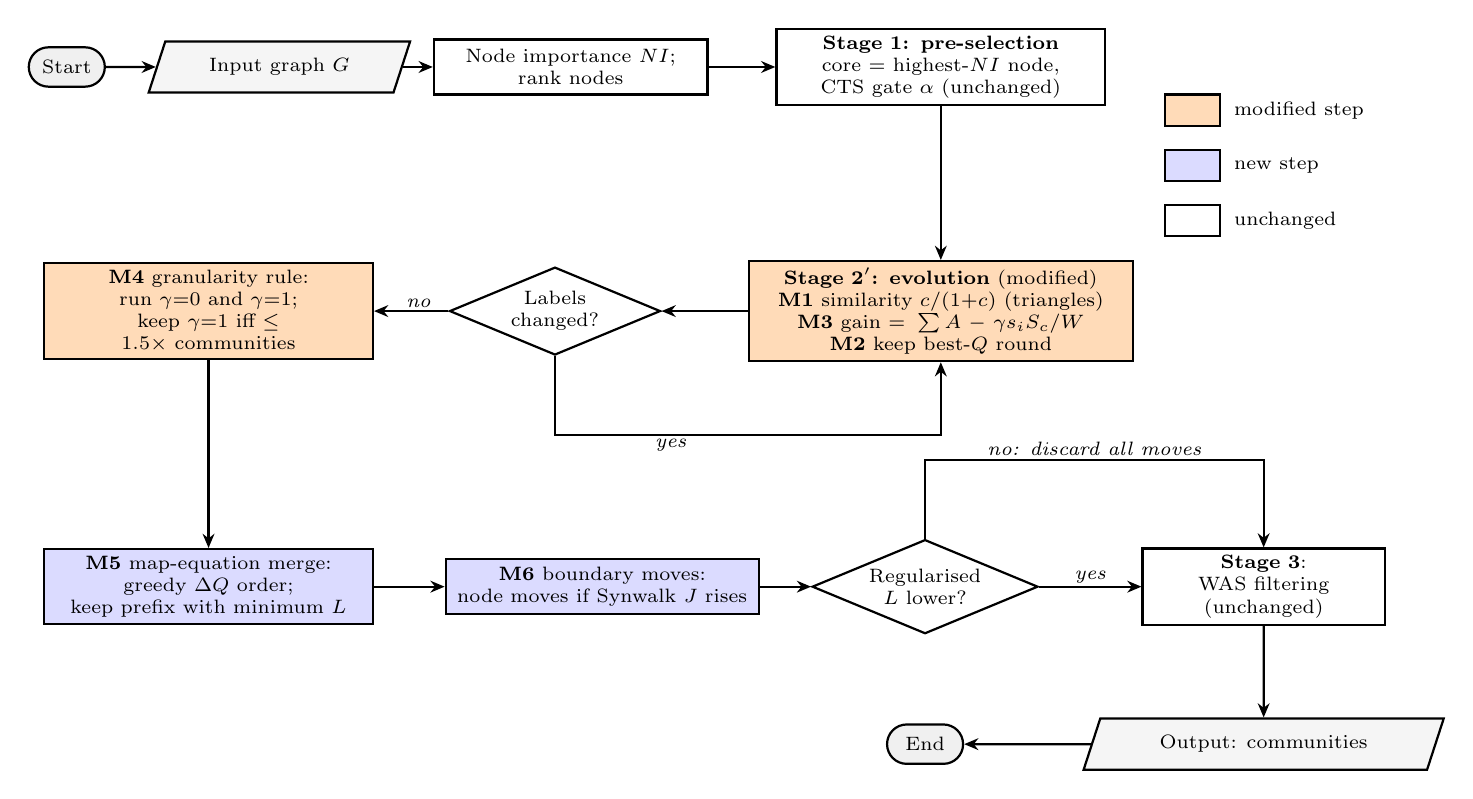
\begin{tikzpicture}[x=1cm,y=1cm]
\node[term] (s) at (0.8,0) {Start};
\node[io] (in) at (3.5,0) {Input graph $G$};
\node[proc, text width=33mm] (ni) at (7.2,0) {Node importance $NI$;\\ rank nodes};
\node[proc, text width=40mm] (s1) at (11.9,0) {\textbf{Stage 1: pre-selection}\\ core = highest-$NI$ node,\\ CTS gate $\alpha$ (unchanged)};
\node[modp, text width=47mm] (s2) at (11.9,-3.1) {\textbf{Stage 2$'$: evolution} (modified)\\ \textbf{M1} similarity $c/(1{+}c)$ (triangles)\\ \textbf{M3} gain $=\sum A-\gamma s_iS_c/W$\\ \textbf{M2} keep best-$Q$ round};
\node[dec] (d2) at (7.0,-3.1) {Labels\\changed?};
\node[modp, text width=40mm] (m4) at (2.6,-3.1) {\textbf{M4} granularity rule:\\ run $\gamma{=}0$ and $\gamma{=}1$;\\ keep $\gamma{=}1$ iff $\le1.5\times$ communities};
\node[newp, text width=40mm] (m5) at (2.6,-6.6) {\textbf{M5} map-equation merge:\\ greedy $\Delta Q$ order;\\ keep prefix with minimum $L$};
\node[newp, text width=38mm] (m6) at (7.6,-6.6) {\textbf{M6} boundary moves:\\ node moves if Synwalk $J$ rises};
\node[dec] (g) at (11.7,-6.6) {Regularised\\$L$ lower?};
\node[proc, text width=29mm] (s3) at (16.0,-6.6) {\textbf{Stage 3}: WAS filtering\\ (unchanged)};
\node[io] (out) at (16.0,-8.6) {Output: communities};
\node[term] (e) at (11.7,-8.6) {End};
\draw[arr] (s)--(in); \draw[arr] (in)--(ni); \draw[arr] (ni)--(s1);
\draw[arr] (s1)--(s2);
\draw[arr] (s2)--(d2);
\draw[arr] (d2.south) -- ++(0,-1.0) -| (s2.south) node[lab, pos=.15, below]{yes};
\draw[arr] (d2)--(m4) node[lab, pos=.4, above]{no};
\draw[arr] (m4)--(m5);
\draw[arr] (m5)--(m6);
\draw[arr] (m6)--(g);
\draw[arr] (g)--(s3) node[lab, pos=.5, above]{yes};
\draw[arr] (g.north) -- ++(0,1.0) -| (s3.north) node[lab, pos=.25, above]{no: discard all moves};
\draw[arr] (s3)--(out); \draw[arr] (out)--(e);
\node[proc, fill=orange!28, minimum width=7mm, minimum height=4mm] at (15.1,-0.55) (l1) {};
\node[font=\scriptsize, anchor=west] at (15.5,-0.55) {modified step};
\node[proc, fill=blue!14, minimum width=7mm, minimum height=4mm] at (15.1,-1.25) (l2) {};
\node[font=\scriptsize, anchor=west] at (15.5,-1.25) {new step};
\node[proc, minimum width=7mm, minimum height=4mm] at (15.1,-1.95) (l3) {};
\node[font=\scriptsize, anchor=west] at (15.5,-1.95) {unchanged};
\end{tikzpicture}
\caption{Architecture of the proposed pipeline. Orange boxes modify a step of TPOC-LPA, blue boxes are new steps, white boxes are unchanged (compare Fig.~\ref{fig:base}).}
\label{fig:ours}
\end{figure*}

\textbf{Preliminaries: the map equation.} Two of the modifications use the map equation~\cite{rosvall2008}, so we introduce it first. Imagine describing the path of a random walker on the graph with as few bits as possible. If the nodes are grouped into modules, each module gets its own short codebook for node names, and one extra code announces a move from one module to another. A partition that matches real communities keeps the walker inside a module most of the time, so the module codebooks are used often and the announcement code rarely, and the description is short. The expected description length per step is the \emph{codelength} $L$. For an undirected graph, with module exit rates $q_i=\mathrm{cut}_i/2m$, module visit rates $p_i=\mathrm{vol}_i/2m$, node visit rates $p_\alpha=k_\alpha/2m$, $q=\sum_iq_i$ and $f(x)=x\log_2x$,
\begin{equation}
L=f(q)-2\sum_if(q_i)+\sum_if(q_i+p_i)-\sum_\alpha f(p_\alpha).\label{eq:L}
\end{equation}
Lower is better. Merging two modules saves the announcements between them but lengthens the codebook of the merged module, so $L$ falls only if the two modules are linked strongly enough; this is why its resolution limit depends on the links between modules and not on the size of the whole graph~\cite{kawamoto2015}. Our implementation reproduces the codelength of the Infomap package (to $10^{-15}$ for this form, and to four decimals for the regularised form below). On sparse graphs $L$ can over-fit; the \emph{regularised} codelength $L_{\mathrm{reg}}$~\cite{smiljanic2020} is the map equation of $G$ plus a complete graph of small weight $\ln N/N$ on every pair of nodes, which stops it from trusting thin local patterns.

\textbf{M1: triangle-based similarity (replaces Jaccard in Eq.~\eqref{eq:A}).} With $c=|N(i)\cap N(j)|$ the number of triangles on edge $(i,j)$,
\begin{equation}
\mathrm{Sim}(i,j)=\frac{c}{1+c}\quad(0\to0,\;1\to0.5,\;3\to0.75,\;9\to0.9),\label{eq:motif}
\end{equation}
which depends on the triangle count and not on the sizes of the neighbourhoods. It costs a little on sparse graphs, where one shared neighbour is often chance but scores 0.5.

\textbf{M2: best-iterate guard.} Let $Q_t$ be the modularity of the labels after Stage~2 round $t$ ($t=0$: the Stage~1 partition). The guard returns the labels of $\argmax_tQ_t$ instead of the last round. It changes nothing unless a later round is worse.

\textbf{M3: size-corrected gain.} Stage~2 scores a candidate community by Eq.~\eqref{eq:gain} with $\gamma=1$. This is LPAm with importance-weighted edges; used alone it fragments graphs whose labels are coarse (Karate, Dolphin, Polbooks), hence M4.

\textbf{M4: granularity rule (selector).} Starting from the same Stage~1 partition we run the paper-style Stage~2 ($\gamma=0$, with M1 and M2) giving $L^{(0)}$, and the corrected one ($\gamma=1$, with M1) giving $L^{(1)}$. With $|L|$ the number of communities,
\begin{equation}
L=\begin{cases}L^{(1)}&\text{if }|L^{(1)}|\le\rho\,|L^{(0)}|,\\ L^{(0)}&\text{otherwise,}\end{cases}\qquad\rho=1.5.\label{eq:gran}
\end{equation}
When both agree on the scale, $\gamma=1$ only fine-tunes boundaries; when it shatters the graph (we measured $|L^{(1)}|/|L^{(0)}|$ of 2.0 for Karate and Dolphin, 2.3 for Polbooks, 5.0 for Polblogs, against $\le1.4$ on Football, Citeseer, Cora and LFR) we are in the coarse-truth case and keep $L^{(0)}$. The test uses no labels. The value $\rho=1.5$ was chosen by leave-one-dataset-out on our development graphs.

\textbf{M5: map-equation merge.} After Stage~2, adjacent communities $a,b$ are merged greedily by the modularity gain
\begin{equation}
\Delta Q(a,b)=\frac{e_{ab}}{m}-\frac{d_ad_b}{2m^2},\label{eq:dq}
\end{equation}
($e_{ab}$: edges between them, $d_a$: volume), using a heap with lazy deletion (stale or outdated entries are skipped or refreshed when popped). The earlier version kept all merges if $\sum\Delta Q\ge0.03$; on SNAP-DBLP it merged 9{,}803 communities into 807 and cut NMI from 0.7667 to 0.6197 because modularity favours merging at the wrong scale. We keep the merge order but evaluate the codelength $L$ (Eq.~\eqref{eq:L}) after every merge (updating only the terms of the two communities, in $O(1)$) and return the \emph{prefix} of merges at which $L$ was lowest; if no prefix lowers $L$, nothing is merged. The map equation is used because its resolution limit depends on the links between modules and not on the size of the graph.

\textbf{M6: boundary moves with a Synwalk score.} The Synwalk objective~\cite{toth2022} is a sum over modules of
\begin{equation}
j(\mathrm{vol},\mathrm{cut})=\frac{\mathrm{vol}-\mathrm{cut}}{2m}\ln\frac{1-\mathrm{cut}/\mathrm{vol}}{\mathrm{vol}/2m}+\frac{\mathrm{cut}}{2m}\ln\frac{\mathrm{cut}/\mathrm{vol}}{1-\mathrm{vol}/2m},\label{eq:synwalk}
\end{equation}
which is the KL divergence between a module's stay/leave probabilities and those of a walker placed at random, weighted by the module's visit rate. Node $i$ of degree $k_i$ in module $a$, with $k_{ia}$ links into $a$ and $k_{ib}$ into a neighbouring module $b$, moving $a\to b$ changes the modules to
\begin{align}
&(\mathrm{vol}_a',\mathrm{cut}_a')=(\mathrm{vol}_a-k_i,\;\mathrm{cut}_a-(k_i-k_{ia})+k_{ia}),\notag\\
&(\mathrm{vol}_b',\mathrm{cut}_b')=(\mathrm{vol}_b+k_i,\;\mathrm{cut}_b+(k_i-k_{ib})-k_{ib}),\label{eq:move}
\end{align}
so a move is scored by recomputing two terms: $\Delta J=j(a')+j(b')-j(a)-j(b)$. Nodes are visited in decreasing $NI$ and each moves to the neighbouring module with the largest positive $\Delta J$; sweeps repeat until no node moves (at most $S=20$). There is no aggregation step, so communities are never joined wholesale. The whole pass is accepted only if the regularised codelength $L_{\mathrm{reg}}$ also falls; otherwise all moves are discarded. The gate exists because the plain map equation over-fits small graphs: one move costs 0.16 NMI on Karate. It was designed after seeing that failure, so it is a post-hoc choice.

\textbf{Stage 3.} Unchanged (Eq.~\eqref{eq:was}), applied to the final partition.

\textbf{Complexity.} Per Stage~2 round, similarities are computed once per edge, and one round scans each edge a constant number of times; the granularity rule runs Stage~2 twice. The merge pass is a heap-driven procedure whose cost is dominated by heap operations over adjacent community pairs; the moves cost $O(S\cdot m)$ at most, since a move scores one candidate per neighbouring module. We have not proved tighter bounds; Table~\ref{tab:time} gives measured times.



%=====================================================================
\section{Experimental Results}\label{sec:results}
\subsection{Setup and Protocol}\label{sec:setup}
\textbf{Methods compared.} Fastgreedy~\cite{clauset2004}, LPA~\cite{raghavan2007}, Louvain~\cite{blondel2008} and Walktrap~\cite{pons2006} (all through the igraph C library), the baseline TPOC-LPA as we re-implemented it (TPOC$^{\dagger}$), and our pipeline (M1--M6). Infomap~\cite{rosvall2008} is not in~\cite{kong2026}; we add it because M5 and M6 borrow from it, so it is the strongest reference. For overlap we compare with SLPA~\cite{xie2011} ($T{=}100$), implemented by us, with $r$ tuned per graph as the paper tunes it. NSA, SimCMR, WLC, UMSTMO, GREESE and MDPA have no public code that we could find, and we did not re-implement them from a paragraph of description; their published numbers are quoted in Table~\ref{tab:paper} and marked as such.

\textbf{Conventions in the tables.} FG = Fastgreedy, Louv. = Louvain, Walk. = Walktrap, Info.$^{*}$ = Infomap (extra baseline) and TPOC$^{\dagger}$ = our re-implementation of TPOC-LPA. Stochastic methods are the mean of 10 runs (3 on the SNAP and LFR graphs); the best value of each row is in bold; ``Mean'' and ``Mean rank'' are taken over the rows shown. SNAP$^{*}$ rows are our own induced subgraphs, with the first listed community as truth. Table~\ref{tab:lfr} uses the settings of Table~\ref{tab:lfrparam} (mean of 5 graphs per row, with $c_{\min}{=}15$ instead of 10 for $n{=}1000$), and Table~\ref{tab:ov} averages $om=2$ to 8 over two generator seeds, with $r$ of SLPA tuned per graph by LFK-NMI, which favours SLPA.

\textbf{Protocol.} We kept development graphs (Karate, Dolphin, Football, Polbooks, Polblogs, email-Eu, Cora, Citeseer, Amazon Photo, LFR $n{=}1000$ seeds 1--5) apart from held-out graphs (72 further LFR variants, Amazon Computers, Coauthor-CS, Coauthor-Physics) and fresh ones used once. A change became a candidate default only if no held-out real graph lost more than 0.005 NMI. Stochastic baselines are averaged over 10 runs (3 on SNAP and LFR); we also computed their best run, which leaves the conclusions unchanged (mean rank on real graphs 2.4 for our pipeline; LFR mean 0.9941 against 0.9931 for Infomap). Our own pipeline and TPOC$^{\dagger}$ are deterministic.

\textbf{NMI normalisation.} The normalisation used in~\cite{kong2026} is not clear to us: for the same Fastgreedy partition of Karate it reports 0.7069 while we obtain 0.5646, and no standard variant reproduces its value. We use one metric implementation for all our columns, so only differences \emph{within} our tables are meaningful.

\subsection{Real Networks}
@@T_REAL@@
Table~\ref{tab:real} gives the main result. The pipeline has the best mean rank (2.00 against 4.09--4.73 for every other column) and the highest mean NMI (0.7031 against 0.6585 for Infomap). Part of this margin comes from email-Eu, where the baseline collapses (0.0000) and our pipeline reaches 0.6677, above Louvain (0.5806) and Infomap (0.5873). On the three graphs shared with~\cite{kong2026} (Karate, Dolphin, Football) it scores 0.8372, 0.9495 and 0.9242, above Infomap (0.5805, 0.8993, 0.8683). On SNAP-DBLP it is marginally ahead (0.7676 against 0.7657 for LPA and 0.7631 for Infomap).

It is not best everywhere. On Cora, Fastgreedy is higher (0.4647 against 0.4192); on SNAP-Amazon, Louvain is (0.9825 against 0.9731); and on \textbf{SNAP-Youtube Infomap (0.7486) and Walktrap (0.7222) are far ahead of our 0.5745}, which is itself better than the baseline's 0.5195.

\subsection{LFR Benchmarks and Ablation}
@@T_LFR@@
Table~\ref{tab:lfr} shows that the mean NMI of our pipeline over the six settings is 0.9941, against 0.9905 for Infomap and 0.9805 for TPOC$^{\dagger}$. At $\mu{=}0.6$ the mean is 0.9883 against 0.9827 for Infomap and 0.9629 for TPOC$^{\dagger}$. Infomap is slightly higher on $n{=}5000$ and $n{=}10000$ at $\mu{=}0.6$ (0.9945 against 0.9940 and 0.9900 against 0.9895), which is within seed noise. The published baseline reports 0.9869 on its own $n{=}1000$, $\mu{=}0.6$ graphs; on our five graphs of that setting TPOC$^{\dagger}$ reaches 0.9317 and our pipeline 0.9815. Table~\ref{tab:abl} shows where the gain comes from; its rows are development runs (15 graphs for each LFR column, one graph for email-Eu) with the merge pass M5 switched off.
@@T_ABL@@
On the 72 held-out synthetic graphs, the configuration with M1--M4 averaged 0.7814 and the final pipeline with M5 and M6 averaged 0.8069, better on 65, equal on 7 and worse on 3 graphs (worst $-0.010$).

\subsection{Overlapping Communities}
@@T_OV@@
Table~\ref{tab:ov} reports overlap quality. With the paper's own WAS Stage~3 on top of our Stage~2, the pipeline has the highest mean LFK-NMI (0.7673 against 0.7578 for tuned SLPA and 0.7600 for TPOC$^{\dagger}$), and it wins R1--R4. It loses R5 and R6 (the 10{,}000-node families) to SLPA, and on the Omega mean SLPA is ahead (0.7571 against 0.7418).

\subsection{Extended Modularity (EQ)}
@@T_EQ@@
Table~\ref{tab:eq}: our pipeline is best on 5 of 12 networks (Jazz, Lesmis, Power, Facebook, LastFM), and SLPA on the other 7; for SLPA the threshold $r$ was scanned from 0.05 to 0.5 and the best EQ kept, so it is tuned on EQ itself. The mean EQ is 0.5920 for ours against 0.6013 for SLPA and 0.5750 for TPOC$^{\dagger}$.

\subsection{Latency and Scalability}\label{sec:latency}
@@LAT_SECTION@@
\subsection{Published Numbers of the Baselines Without Public Code}
@@T_PAPER@@
Table~\ref{tab:paper} lists the values published in~\cite{kong2026}, including the two baselines (NSA and SimCMR) for which we found no implementation. They are not comparable with Tables~\ref{tab:real} and~\ref{tab:lfr}, because the NMI normalisation and the graph instances differ.

%=====================================================================
\section{Discussion}\label{sec:discussion}
\subsection{What Drives the Gains}
The gains come from different modifications on different graphs (Table~\ref{tab:abl}). M1--M4 remove the collapse: email-Eu goes from 0.0000 to 0.6381 and LFR $\mu{=}0.7$ from 0.0513 to 0.8534. M6 adds a second, smaller gain on the high-mixing LFR graphs and on email-Eu (LFR $\mu{=}0.6$: $0.9637\to0.9830$), consistent with its role of repairing boundary nodes, which is the error that remains after Stage~2. The Synwalk score beats the map-equation score on these graphs (0.9830 against 0.9776 at $\mu{=}0.6$, 0.8917 against 0.8759 at $\mu{=}0.7$), in line with the reported advantage of Synwalk at high mixing, but it is slightly worse on coarse and sparse real graphs. M5 matters on large sparse graphs: the modularity merge reduced NMI on SNAP-DBLP by 0.147 and on fresh sparse LFR graphs by 0.12--0.23, while the map-equation stop changed it by between $-0.008$ and $+0.005$.

\subsection{Where the Pipeline Loses}
\textbf{SNAP-Youtube.} The ground truth has 4{,}447 communities. The two methods that return many communities are far ahead: Infomap returns about 2{,}345 (NMI 0.7486) and Walktrap 4{,}567 (0.7222). Every method that returns 955 to 1{,}389 communities scores between 0.50 and 0.57: Louvain about 955 (0.5410), LPA about 1{,}202 (0.5040), our pipeline 1{,}209 (0.5745), Fastgreedy 1{,}262 (0.5212) and TPOC$^{\dagger}$ 1{,}389 (0.5195). Our pipeline returns fewer communities than TPOC$^{\dagger}$, so the merge and move steps reduce the count further. This is consistent with Youtube having many small communities that a coarser partition combines, but we have not tested it; it remains an open problem.

\textbf{Sparse graphs with coarse labels.} On Cora and Citeseer the pipeline is no better than the baseline (0.4192 against 0.4192; 0.3438 against 0.3465), and the moves cost up to 0.008 on sparse real graphs. On graphs whose labels are coarse (Coauthor-Physics, Coauthor-CS, Cora) a modularity merge scores higher than the map-equation stop (Physics 0.4324 against 0.2790) because the resolution limit of modularity happens to match the coarse labels; no label-free criterion that we tried could tell this case from fine-grained truth, and every candidate (a map-equation guard, a Synwalk guard, relative-codelength vetoes) failed on some graph.

\textbf{Karate.} Our NMI of 0.8372 stays below the 1.0000 reported in~\cite{kong2026}: node 8 has three links to the other faction and two to its own, so any structure-only rule assigns it the other way, and the plain LPA baseline in the same paper also scores 0.8372. We also found that networkx's Karate graph carries edge weights; on the unweighted graph our partition has $Q=0.3715$, which equals the $Q$ reported in~\cite{kong2026}, whereas the true two-faction split has $Q=0.3582$. This suggests that the reported $Q$ and NMI do not come from the same partition, but we cannot prove it.

\subsection{Overlap}
The overlap result is the weakest part. Our re-implemented baseline scores below the values published for TPOC-LPA on the same families (for instance 0.7949 against 0.8358 for R1 under LFK-NMI), and we could not close that gap. We decomposed the loss on R1 and R2: given our Stage~2 partition, a \emph{perfect} Stage~3 would reach LFK-NMI 0.84--0.98, so most of the loss is in Stage~3. But the missing memberships are mostly nodes with a single link into the other community, and such a link is a true membership only 7--11\% of the time, so no local rule can find them; a rule based on triangles closed inside the candidate community had precision 0.92--0.99 on R1 (three or more embedded links) but found too few memberships and added nothing to WAS. The EQ result is mixed: tuned SLPA is competitive on EQ (and its $r$ is tuned on EQ itself), and we did not investigate the gap further.

\subsection{Failed Ideas}\label{sec:neg}
These were tried and dropped; they remain in the code as ``explored, not adopted''.
\begin{itemize}
\item \emph{LLM correction of Stage~2} with local 3--8B models. Oracle headroom exists (Football $+0.059$), but a hard override with the measured accuracy of 0.817 gave NMI 0.7815 against 0.9095 structure-only.
\item \emph{Map-equation guard in place of modularity (M2):} email-Eu fell from 0.64 to 0.00, because the map equation prefers one module when structure is weak.
\item \emph{Persona (ego-splitting) Stage~3:} it matched the published overlap numbers on our design graphs and helped on held-out synthetic ones, but lost on real graphs (SNAP-Amazon $-0.009$, SNAP-DBLP $-0.015$ $\mathrm{NMI}_{\max}$ against the best WAS).
\item \emph{Near-tie and embedded-link overlap rules:} they help SNAP-DBLP only, or add nothing once WAS is applied.
\item \emph{Selecting $\alpha$ by codelength,} link-majority polishing and consensus clustering did not pass the held-out test.
\end{itemize}

\subsection{Threats to Validity}\label{sec:limits}
\begin{itemize}
\item \textbf{Post-hoc choices.} $\rho=1.5$ (picked on development data), the regularised gate in M6, $s=3$ for personas, and $\beta=0.8$ taken from the paper. A choice made after seeing development data may not transfer.
\item \textbf{No universal improvement.} All modifications remain opt-in; Coauthor-CS and Coauthor-Physics fail our adoption rule.
\item \textbf{Different graphs and metric.} SNAP subgraphs and the NMI normalisation differ from those of~\cite{kong2026}; cross-paper numbers are indicative only, and we could not reproduce its overlapping-LFR and EQ values for our baseline implementation.
\item \textbf{Baselines.} Six baselines of the paper are not re-run, Leiden is not included, and SLPA is tuned with the labels, which favours it. The overlap result rests on two generator seeds.
\item \textbf{Novelty.} Each component exists in prior work; the contribution is the analysis of where TPOC-LPA fails, the combination and the gates, and the comparison.
\end{itemize}

%=====================================================================
\section{Conclusion}
We re-implemented TPOC-LPA, identified an unnormalised size effect in its Stage~2 that explains its collapse on dense graphs and under-merging on sparse ones, and added six optional modifications that keep the published behaviour as the default: a triangle similarity, a best-iterate guard, a size-corrected gain with a label-free granularity rule, a merge pass stopped by the map equation, and boundary moves scored by the Synwalk objective and accepted through a regularised gate. Compared with baselines re-run on identical graphs, the pipeline has the best mean rank on real networks and the highest mean NMI on LFR, repairs the collapse on dense graphs, and is competitive on overlap, but it is far behind Infomap on SNAP-Youtube, behind SLPA on the largest overlapping benchmarks and below the published EQ values; it is about 25\% slower than our baseline re-implementation, and both are far slower than the C implementations of the other methods.

\textbf{Future work.} (i) Diagnose the Youtube gap, starting from the number of communities. (ii) Calibrate the overlap rate without labels. (iii) Add Leiden and, if code is released, the six baselines we could not run. (iv) Test the pipeline on more fresh graphs before proposing any of the changes as defaults.

\begin{thebibliography}{00}
\bibitem{kong2026} Z. Kong, Y. Huo, Y. Wang and Y. Guo, ``Three-stage overlapping community detection algorithm based on label propagation,'' \emph{Expert Syst. Appl.}, vol.~317, art.~131873, 2026. \url{https://doi.org/10.1016/j.eswa.2026.131873}
\bibitem{girvan2002} M. Girvan and M. E. J. Newman, ``Community structure in social and biological networks,'' \emph{Proc. Natl. Acad. Sci. USA}, vol.~99, no.~12, pp.~7821--7826, 2002. \url{https://doi.org/10.1073/pnas.122653799}
\bibitem{fortunato2010} S. Fortunato, ``Community detection in graphs,'' \emph{Phys. Rep.}, vol.~486, nos.~3--5, pp.~75--174, 2010. \url{https://doi.org/10.1016/j.physrep.2009.11.002}
\bibitem{newman2004} M. E. J. Newman and M. Girvan, ``Finding and evaluating community structure in networks,'' \emph{Phys. Rev. E}, vol.~69, 026113, 2004. \url{https://doi.org/10.1103/physreve.69.026113}
\bibitem{raghavan2007} U. N. Raghavan, R. Albert and S. Kumara, ``Near linear time algorithm to detect community structures in large-scale networks,'' \emph{Phys. Rev. E}, vol.~76, 036106, 2007. \url{https://doi.org/10.1103/physreve.76.036106}
\bibitem{leung2009} I. X. Y. Leung, P. Hui, P. Li\`o and J. Crowcroft, ``Towards real-time community detection in large networks,'' \emph{Phys. Rev. E}, vol.~79, 066107, 2009. \url{https://doi.org/10.1103/physreve.79.066107}
\bibitem{traag2023} V. A. Traag and L. \v{S}ubelj, ``Large network community detection by fast label propagation,'' \emph{Sci. Rep.}, vol.~13, 2701, 2023. \url{https://doi.org/10.1038/s41598-023-29610-z}
\bibitem{barber2009} M. J. Barber and J. W. Clark, ``Detecting network communities by propagating labels under constraints,'' \emph{Phys. Rev. E}, vol.~80, 026129, 2009. \url{https://doi.org/10.1103/physreve.80.026129}
\bibitem{liu2010} X. Liu and T. Murata, ``Advanced modularity-specialized label propagation algorithm for detecting communities in networks,'' \emph{Physica A}, vol.~389, no.~7, pp.~1493--1500, 2010. \url{https://doi.org/10.1016/j.physa.2009.12.019}
\bibitem{clauset2004} A. Clauset, M. E. J. Newman and C. Moore, ``Finding community structure in very large networks,'' \emph{Phys. Rev. E}, vol.~70, 066111, 2004. \url{https://doi.org/10.1103/physreve.70.066111}
\bibitem{blondel2008} V. D. Blondel, J.-L. Guillaume, R. Lambiotte and E. Lefebvre, ``Fast unfolding of communities in large networks,'' \emph{J. Stat. Mech.}, P10008, 2008. \url{https://doi.org/10.1088/1742-5468/2008/10/p10008}
\bibitem{traag2019} V. A. Traag, L. Waltman and N. J. van Eck, ``From Louvain to Leiden: guaranteeing well-connected communities,'' \emph{Sci. Rep.}, vol.~9, 5233, 2019. \url{https://doi.org/10.1038/s41598-019-41695-z}
\bibitem{pons2006} P. Pons and M. Latapy, ``Computing communities in large networks using random walks,'' \emph{J. Graph Algorithms Appl.}, vol.~10, no.~2, pp.~191--218, 2006. \url{https://doi.org/10.7155/jgaa.00124}
\bibitem{rosvall2008} M. Rosvall and C. T. Bergstrom, ``Maps of random walks on complex networks reveal community structure,'' \emph{Proc. Natl. Acad. Sci. USA}, vol.~105, no.~4, pp.~1118--1123, 2008. \url{https://doi.org/10.1073/pnas.0706851105}
\bibitem{lancichinetti2009cmp} A. Lancichinetti and S. Fortunato, ``Community detection algorithms: a comparative analysis,'' \emph{Phys. Rev. E}, vol.~80, 056117, 2009. \url{https://doi.org/10.1103/physreve.80.056117}
\bibitem{fortunato2007} S. Fortunato and M. Barth\'elemy, ``Resolution limit in community detection,'' \emph{Proc. Natl. Acad. Sci. USA}, vol.~104, no.~1, pp.~36--41, 2007. \url{https://doi.org/10.1073/pnas.0605965104}
\bibitem{kawamoto2015} T. Kawamoto and M. Rosvall, ``Estimating the resolution limit of the map equation in community detection,'' \emph{Phys. Rev. E}, vol.~91, 012809, 2015. \url{https://doi.org/10.1103/physreve.91.012809}
\bibitem{smiljanic2020} J. Smiljani\'c, D. Edler and M. Rosvall, ``Mapping flows on sparse networks with missing links,'' \emph{Phys. Rev. E}, vol.~102, 012302, 2020. \url{https://doi.org/10.1103/physreve.102.012302}
\bibitem{toth2022} C. Toth, D. Helic and B. C. Geiger, ``Synwalk -- community detection via random walk modelling,'' \emph{Data Min. Knowl. Discov.}, vol.~36, no.~2, pp.~739--780, 2022. \url{https://doi.org/10.1007/s10618-021-00809-w}
\bibitem{li2020motif} P.-Z. Li, L. Huang, C.-D. Wang, J.-H. Lai and D. Huang, ``Community detection by motif-aware label propagation,'' \emph{ACM Trans. Knowl. Discov. Data}, vol.~14, no.~2, 2020. \url{https://doi.org/10.1145/3378537}
\bibitem{palla2005} G. Palla, I. Der\'enyi, I. Farkas and T. Vicsek, ``Uncovering the overlapping community structure of complex networks in nature and society,'' \emph{Nature}, vol.~435, pp.~814--818, 2005. \url{https://doi.org/10.1038/nature03607}
\bibitem{xie2011} J. Xie, B. K. Szymanski and X. Liu, ``SLPA: Uncovering overlapping communities in social networks via a speaker-listener interaction dynamic process,'' in \emph{Proc. IEEE ICDM Workshops}, 2011. \url{https://doi.org/10.1109/icdmw.2011.154}
\bibitem{gregory2010} S. Gregory, ``Finding overlapping communities in networks by label propagation,'' \emph{New J. Phys.}, vol.~12, 103018, 2010. \url{https://doi.org/10.1088/1367-2630/12/10/103018}
\bibitem{epasto2017} A. Epasto, S. Lattanzi and R. Paes Leme, ``Ego-splitting framework: from non-overlapping to overlapping clusters,'' in \emph{Proc. ACM KDD}, 2017. \url{https://doi.org/10.1145/3097983.3098054}
\bibitem{lfr2008} A. Lancichinetti, S. Fortunato and F. Radicchi, ``Benchmark graphs for testing community detection algorithms,'' \emph{Phys. Rev. E}, vol.~78, 046110, 2008. \url{https://doi.org/10.1103/physreve.78.046110}
\bibitem{lfk2009} A. Lancichinetti, S. Fortunato and J. Kert\'esz, ``Detecting the overlapping and hierarchical community structure in complex networks,'' \emph{New J. Phys.}, vol.~11, 033015, 2009. \url{https://doi.org/10.1088/1367-2630/11/3/033015}
\bibitem{collins1988} L. M. Collins and C. W. Dent, ``Omega: a general formulation of the Rand index of cluster recovery suitable for non-disjoint solutions,'' \emph{Multivariate Behav. Res.}, vol.~23, no.~2, pp.~231--242, 1988. \url{https://doi.org/10.1207/s15327906mbr2302_6}
\bibitem{shen2009} H. Shen, X. Cheng, K. Cai and M.-B. Hu, ``Detect overlapping and hierarchical community structure in networks,'' \emph{Physica A}, vol.~388, no.~8, pp.~1706--1712, 2009. \url{https://doi.org/10.1016/j.physa.2008.12.021}
\bibitem{yang2012} J. Yang and J. Leskovec, ``Defining and evaluating network communities based on ground-truth,'' in \emph{Proc. IEEE ICDM}, 2012. \url{https://doi.org/10.1109/icdm.2012.138}
\bibitem{zachary1977} W. W. Zachary, ``An information flow model for conflict and fission in small groups,'' \emph{J. Anthropol. Res.}, vol.~33, no.~4, pp.~452--473, 1977. \url{https://doi.org/10.1086/jar.33.4.3629752}
\bibitem{lusseau2003} D. Lusseau \emph{et al.}, ``The bottlenose dolphin community of Doubtful Sound features a large proportion of long-lasting associations,'' \emph{Behav. Ecol. Sociobiol.}, vol.~54, pp.~396--405, 2003. \url{https://doi.org/10.1007/s00265-003-0651-y}
\bibitem{adamic2005} L. A. Adamic and N. Glance, ``The political blogosphere and the 2004 U.S. election: divided they blog,'' in \emph{Proc. 3rd Int. Workshop on Link Discovery}, 2005. \url{https://doi.org/10.1145/1134271.1134277}
\bibitem{yin2017} H. Yin, A. R. Benson, J. Leskovec and D. F. Gleich, ``Local higher-order graph clustering,'' in \emph{Proc. ACM KDD}, 2017. \url{https://doi.org/10.1145/3097983.3098069}
\bibitem{sen2008} P. Sen, G. Namata, M. Bilgic, L. Getoor, B. Galligher and T. Eliassi-Rad, ``Collective classification in network data,'' \emph{AI Mag.}, vol.~29, no.~3, pp.~93--106, 2008. \url{https://doi.org/10.1609/aimag.v29i3.2157}
\end{thebibliography}
\end{document}
